% Part 1, closing chapters (2 of 2): the thermodynamic identity of the kinetic half.
% Carried line by line from: The Thermodynamic Identity Governing the Virial Theorem: Physical Identification of K and Evidence Across 37 Orders of
% Magnitude (PRL version, 18 Mar 2026; all sections); The Virial Partition from Atoms to the Horizon (Oct 2026; section 5);
% The Virial Partition Across Wide Range of Physical Scales (25 Feb 2026; section 2.3, steps 1-3).
% Corrections applied: errata V1, V2, V13, V18, V19, V29, EM1; VIRIAL_CHECK.md items 1, 13 and the 'What stands' note on the temperature of step 2.
% Numbers: docs/verification/scripts/verify_virial_papers.py (sections B, F) and verify_virial_atoms_to_horizon.py.

\chapter{What the kinetic half is: the thermodynamic identity}\label{ch:virial_identity}

\section*{Overview}
The virial theorem, established by Clausius in 1870, states that for any stable bound system under a $1/r$ potential, $2\langle K\rangle+\langle V\rangle=0$.
The theorem has been tested across 33 orders of magnitude in the scale of the systems it describes, from the atom to the galaxy cluster, and the cosmological coupling carries it to the horizon, 37 orders (Chapter~\ref{ch:virial_law}), but the physical meaning
of $K$ beyond ``average kinetic energy of bound particles'' has remained unexplained. This chapter shows that the virial theorem and Landauer's principle
are two expressions of the same thermodynamic identity. The first law gives the heat released at the virialization boundary, $Q=-E_f$; the second law and
Landauer's principle give $E_{\rm Landauer}=Q$; the equilibrium condition of the $1/r$ potential gives $-E_f=\langle K\rangle$. Together these identify
$\langle K\rangle$ as the Landauer cost of the virialization transition, encoded onto the nearest available surface as entropy at cost $k_BT\ln2$ per bit.
The virial theorem is the mechanical expression of this thermodynamic identity. The identity is consistent with data across 37 orders of magnitude in
physical scale. In the terms of Chapter~\ref{ch:iams_law} it is IAM's Law operating at the boundary of every $1/r$ bound state; the virial
theorem is its mechanical special case.

\section{What is $K$?}\label{sec:vi_question}
The virial theorem has governed bound systems since Clausius~\cite{Clausius1870}:
\begin{equation}
2\langle K\rangle+\langle V\rangle=0,\qquad\langle K\rangle=\tfrac12|\langle V\rangle|,\label{eq:vi_virial}
\end{equation}
verified from the hydrogen atom ($10^{-10}$\,m) to galaxy clusters ($10^{23}$\,m), and carried by the cosmological coupling to the horizon
($10^{26}$\,m). It is one of the most broadly tested results in physics.

Yet a question has gone unanswered for more than 150 years: what is $K$?

Clausius derived Eq.~\eqref{eq:vi_virial} from Newton's second law. The derivation is mechanical and describes the equilibrium state. It is silent on the
thermodynamic content of the transition that produces the equilibrium, and silent on the physical identity of the energy released during that transition.
The thermodynamics of gravitational systems has been studied extensively (Lynden-Bell \& Wood 1968~\cite{LyndenBellWood1968}; Padmanabhan
1990~\cite{Padmanabhan1990}), but what has not been shown is that the virial theorem and Landauer's principle~\cite{Landauer1961} are two expressions of the same
identity, and that this identity provides the physical meaning of $\langle K\rangle$ as the Landauer cost of the virialization transition itself.

We show this here. The argument proceeds in four steps from principles every physicist accepts: the first law, the second law, Landauer's principle, and
the equilibrium condition of the $1/r$ potential.

\section{Derivation}\label{sec:vi_derivation}

\begin{figure}[htbp]\centering
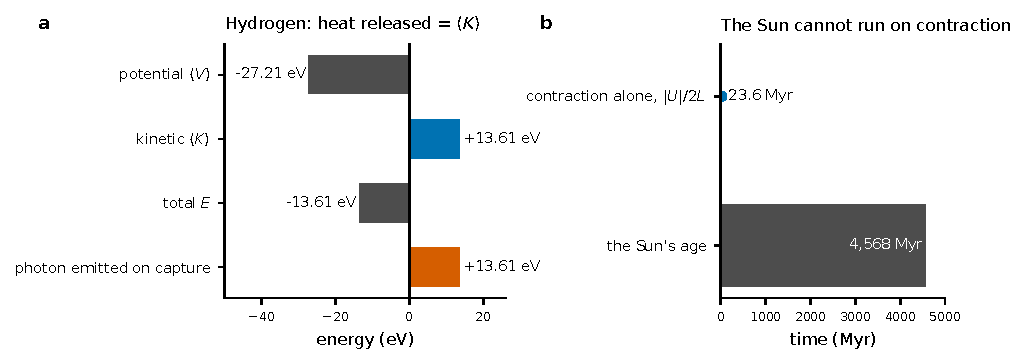
\includegraphics[width=\textwidth]{figures/part1/fig_binding_ledger.pdf}
\caption{(a) Hydrogen captured from rest into the ground state: $\langle V\rangle=-27.21$\,eV, $\langle K\rangle=+13.61$\,eV, $E=-13.61$\,eV, and the photon carries away 13.61\,eV, the kinetic half. (b) The Sun: the energy its contraction alone could radiate, $|U|/2$ with $U=-3GM^2/2R$ ($n=3$ polytrope), lasts $|U|/2L=23.6$\,Myr, against an age of 4,568\,Myr~\cite{Bouvier2010}. CODATA 2018; \texttt{docs/verification/scripts/\allowbreak{}verify\_virial\_atoms\_to\_horizon.py}. \calc}\label{fig:binding_ledger}
\end{figure}

\paragraph{Setup.} Consider a system of total mass $M$ transitioning from an unbound state to a stable bound state under a $1/r$ potential. The natural
reference state is the unbound system at rest at infinity, with $E_i=0$. The bound equilibrium state has total energy
$E_f=\langle K\rangle+\langle V\rangle<0$.

\paragraph{Step 1 (first law).} The transition from unbound to bound is irreversible: a virialized system does not spontaneously return to the unbound
state. The heat released irreversibly to the environment is
\begin{equation}
Q=E_i-E_f=-(\langle K\rangle+\langle V\rangle).\label{eq:vi_Q}
\end{equation}
This is exact. $Q>0$ because $E_f<0$ for any stable bound state. It holds where the binding energy is released to the surroundings: the photon of atomic
recombination, the radiation of a contracting gas cloud or star.

\paragraph{Step 2 (second law).} The irreversible transition produces entropy in the surroundings that receive the heat, at their temperature $T$:
\begin{equation}
\Delta S\ge Q/T .\label{eq:vi_dS}
\end{equation}

\paragraph{Step 3 (Landauer).} By Landauer's principle~\cite{Landauer1961}, the minimum thermodynamic cost of producing entropy $\Delta S$ irreversibly is
$E_{\rm Landauer}=T\Delta S$. The bound is met when $\Delta S=Q/T$, and then
\begin{equation}
E_{\rm Landauer}=T\times\frac QT=Q .\label{eq:vi_EL}
\end{equation}
The temperature cancels exactly. The Landauer cost equals the heat released at the boundary, independently of the scale or temperature of the system.
This step is an identity once the bound is met: it gives no new mechanics, and it gives the released heat its thermodynamic meaning.

\paragraph{Step 4 ($1/r$ equilibrium condition).} Steps 1--3 establish $E_{\rm Landauer}=Q=-E_f$. For a potential $V\propto r^{-1}$, Euler's theorem for
homogeneous functions of degree $-1$ requires $2\langle K\rangle+\langle V\rangle=0$ at stable bound equilibrium, which gives $-E_f=\langle K\rangle$. This is the
equilibrium condition of the $1/r$ potential --- the condition that defines what it means for such a system to be stably bound. Combining with
Eqs.~\eqref{eq:vi_Q} and~\eqref{eq:vi_EL}:
\begin{equation}
\boxed{\;\langle K\rangle=Q=T\Delta S_{\min}=E_{\rm Landauer}=\tfrac12|\langle V\rangle|\;}\label{eq:vi_identity}
\end{equation}
\derived\ (sympy check: \texttt{verify\_virial\_papers.py}, section F).

\paragraph{Remark.} This is not a derivation of the virial theorem from thermodynamics alone: $\langle K\rangle=Q$ follows from the first law and Step 4
alone, which is mechanics. It is the demonstration that the virial theorem and Landauer's principle are two expressions of the same identity: the $1/r$
equilibrium condition gives the mechanical ratio; Landauer's principle identifies the physical content of that ratio as the irreversible thermodynamic cost
of the virialization transition, carried off to the surroundings and recorded there as entropy at $k_BT\ln2$ per bit. \interp\ The $1/2$ partition is not a
free choice: the degree of the potential fixes it, and the identity gives it its thermodynamic meaning.

\paragraph{Hydrogen.} The hydrogen atom shows it directly: an electron captured from rest into the ground state emits a 13.6\,eV photon, the binding
energy, which equals the electron's mean kinetic energy in that state; the potential energy is $-27.2$\,eV (Figure~\ref{fig:binding_ledger}a). The energy
carried away when a $1/r$ system binds equals its kinetic half. \calc

\section{The thermodynamic identity: formal statement}\label{sec:vi_statement}
As a system crosses from an unbound to a bound state under a $1/r$ potential, it releases heat $Q$ irreversibly at the boundary. The first law, the second
law, Landauer's principle, and the equilibrium condition of the $1/r$ potential together require $\langle K\rangle=Q=T\Delta S=E_{\rm Landauer}$. The heat
$Q$ is encoded onto the nearest available surface as entropy at thermodynamic cost $k_BT\ln2$ per bit. The virial theorem $2\langle K\rangle+\langle
V\rangle=0$ is the mechanical expression of this condition. A stable bound state exists if and only if both are satisfied simultaneously. \interp

The scale-invariance of the identity follows directly from the scale-invariance of Landauer's principle: the principle applies wherever an irreversible
process produces entropy, at any scale or temperature. \interp

\paragraph{Scope.} The identity applies wherever the binding energy is released --- the photon of atomic recombination, the radiation of a contracting
cloud or star. A collisionless system (a dark-matter halo) relaxes without radiating; there the half describes the redistribution of energy in violent
relaxation, and the thermodynamic reading concerns the information written in that relaxation, not emitted heat. This is the step IAM takes at
cosmological scale (Chapter~\ref{ch:virial}). \interp

\section{From the hydrogen atom to the cosmological coupling}\label{sec:vi_chain}
The derivation connecting the hydrogen atom to $\beta_m$ proceeds in four steps; the first three are stated here and the fourth opens Part~\ref{part:2}.
\begin{enumerate}
\item \emph{Atomic.} For the Coulomb $1/r$ potential in hydrogen, the virial theorem gives $T=\tfrac12|U|$. Half the magnitude of the binding potential
energy is kinetic (electron motion) and the binding energy released, $|E|=T$, equals it. \derived
\item \emph{Gravitational.} For the gravitational $1/r$ potential in virialized halos, the same theorem gives $K=\tfrac12|U|$. Half the gravitational
energy is kinetic (matter motion) and half is held in the configuration (matter distribution). \derived
\item \emph{Informational.} IAM reads the two halves as two ledgers: $K/(k_BT\ln2)$ counts bits produced by temporal evolution (gravitational decoherence
events); the configuration half, $|U|/2$ in the same units, counts bits stored in spatial configuration. The Landauer energy $E_{\rm bit}=k_BT\ln2$
converts energy to information~\cite{Landauer1961}. \interp
\item \emph{Cosmological.} Applied to structure formation, the kinetic half fixes the coupling of the record term in the horizon first law, $\beta_m=\Omega_m/2$
(Chapter~\ref{ch:virial}). \prediction
\end{enumerate}

\section{Evidence across 37 orders of magnitude}\label{sec:vi_evidence}
Table~\ref{tab:virial_domains} presents the evidence for the thermodynamic identity $\langle K\rangle=Q=\tfrac12|\langle V\rangle|$ across every physical
domain in which bound systems under $1/r$ potentials have been tested. The range spans 37 decades in physical scale, from the atom to the cosmic horizon; the measured rows run from the atom to the galaxy cluster (33 decades),
and the horizon row is the prediction. \calc

The electron mass entry uses the thermodynamic identity applied at the Compton scale: rest energy equals the Landauer cost of maintaining the particle's
decoherence loop at the Gibbons--Hawking temperature of the cosmic horizon. The prediction uses $\hbar$, $H_0$, $m_P$ and $\alpha$ and one factor, $(2\pi)^{3/10}$, that was found by numerical search \fitted;
it agrees with the measured mass to within the $0.3\,\%$ set by the uncertainty of $H_0$ (Chapter~\ref{ch:electronmass}). \conjecture

The atomic and molecular entries use published Hartree--Fock limit energies~\cite{ClementiRoetti1974,Bunge1993}: the mean virial ratio $\eta=-T/E=1.0000000000$
with standard deviation zero across all 20 elements and 10 molecules, that is $T/|V|=1/2$. For converged Hartree--Fock wavefunctions this is analytically
exact, not a numerical coincidence. \calc

The simulated-halo entry compiles the published virial ratios of cosmological N-body halos: $2T/|U|\approx1.1$--$1.3$ within the virial radius
(Bett et al.\ 2007~\cite{Bett2007}; Neto et al.\ 2007~\cite{Neto2007}; Power, Knebe \& Knollmann 2012~\cite{Power2012}), $1.02$--$1.17$ with the
surface-pressure term (Klypin et al.\ 2016~\cite{Klypin2016}), covering halo masses $10^{10}$--$10^{15}\,M_\odot$ with different simulation codes and
analysis pipelines. \observed\ The simulated halos sit at the virial equilibrium to within the infall still under way; how the collapsed fraction and the
relaxed share of the real ensemble of halos combine to the half is set out in Chapter~\ref{ch:virial}.

The cosmological entry instantiates the thermodynamic identity at cosmic scales via IAM, deriving
$\beta_m=\Omega_m/2=0.15765$ from the same $1/2$ partition with no fitted parameters. $\beta_m$ is held fixed at this value in every IAM chain run against
the Planck likelihood (Level~1 as the MGCAMB amplitude $\mu_0=-0.13495$); only the four free-$\mu_0$ test chains sample the amplitude. The Level~2 posterior $\Omega_m=0.3166\pm0.0065$ gives
$\beta_m/\Omega_m=0.498\pm0.010$, and the modified growth is consistent with Planck ($\Delta\chi^2=+0.54$; Chapter~\ref{ch:virial}). \measured

\section{Relationship to Jacobson 1995}\label{sec:vi_jacobson}
Jacobson~\cite{Jacobson1995} derived the Einstein field equations from $\delta Q=T\,\delta S$ applied to the Rindler horizon of an accelerated observer.
That derivation showed that the field equations are thermodynamic in origin. The identity of this chapter applies the same relation $Q=T\Delta S$ to the
virialization boundary and establishes that the virial theorem is its mechanical expression. Both start from the same thermodynamic identity. The present
step extends the Jacobson programme from the field equations governing curved spacetime to the equilibrium condition governing bound states within that
spacetime. \interp\ The thermodynamic framework of Jacobson~\cite{Jacobson1995} is the foundation upon which this work is built.

\section{Conclusion}\label{sec:vi_conclusion}
The virial theorem $2\langle K\rangle+\langle V\rangle=0$ has been tested across 33 orders of magnitude, from the atom to the galaxy cluster, for more than 150 years without a physical
identification of $\langle K\rangle$ beyond ``average kinetic energy of bound particles.'' \observed

The first law, the second law, Landauer's principle, and the equilibrium condition of the $1/r$ potential together establish $\langle K\rangle=Q=T\Delta
S=E_{\rm Landauer}$: the kinetic energy of a virialized system is the Landauer cost of the virialization transition, encoded permanently as entropy on the
nearest available surface. The virial theorem is the mechanical expression of this thermodynamic identity. \interp

The $1/2$ partition is not a numerical coincidence. It is fixed by the degree of the potential, which three-dimensional space fixes, and its thermodynamic
content is the same at every scale. Its appearance across 37 orders of magnitude is a consequence of the scale-invariance of Landauer's principle and the
universality of the $1/r$ potential form. \interp

This thermodynamic identity is IAM's Law at the boundary of a bound state; the virial theorem is its mechanical special case. \interp

Every input behind this identity is public. A physicist can take any bound system in a $1/r$ potential, compute the kinetic half, and follow its cost to the surface where it is paid. That is the thread the rest of the book pulls.
